% File: design.tex
% Date: Sat Jun 22 17:26:42 2013 +0800
% Author: Yuxin Wu <ppwwyyxxc@gmail.com>

\section{项目设计}
项目的目录结构大致如下:
\dirtree{%
  .1 /.
  .2 report/\DTcomment{本报告的\LaTeX 源代码}.
  .2 demo/\DTcomment{一些演示}.
  .2 resource/\DTcomment{程序使用到的外部资源}.
  .2 src/\DTcomment{程序源代码}.
  .3 include/\DTcomment{头文件}.
  .4 geometry/\DTcomment{实现抽象几何对象}.
  .4 renderable/\DTcomment{定义可渲染几何对象}.
  .4 lib/\DTcomment{程序使用的辅助函数定义}.
  .4 material/\DTcomment{实现表面属性及纹理}.
  .4 render/\DTcomment{定义图像渲染}.
  .3 lib/\DTcomment{辅助函数的实现}.
  .4 debugutils.cc.
  .4 utils.cc.
  .4 imagereader.cc.
  .4 Timer.cc.
  .3 renderable/\DTcomment{可渲染几何对象及其渲染相关操作的实现}.
  .4 face.cc.
  .4 mesh.cc.
  .4 plane.cc.
  .4 sphere.cc.
  .3 gui/\DTcomment{图形界面}.
  .4 main.cxx.
  .4 window.cxx.
  .4 window.hh.
  .4 window.ui.
  .4 objviewer.pro.
  .3 kdtree.cc.
  .3 cvrender.cc.
  .3 mesh\_simplifier.cc.
  .3 space.cc.
  .3 static\_const.cc.
  .3 view.cc.
  .3 main.cc.
  .3 Makefile.
  .3 Doxyfile.
}

\subsection{C++类设计}
\begin{enumerate}
  \item 渲染物体相关类的设计

    所有可渲染物体,包括平面、球、面片、网格、KD树,均继承自\verb|Renderable|基类,当其需要与光线求交时,
    通过\verb|Renderable::get_trace()|返回一个\verb|Trace|类的子类对象指针,由
    \verb|Trace|类完成求交相关的操作.一个\verb|Trace|对象相当于一个物体与一条光线的组合.

    \begin{figure}[H]
      \begin{minipage}[b]{0.46\linewidth}
        \centering
        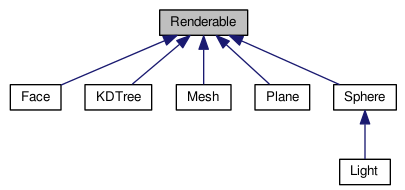
\includegraphics[width=\textwidth]{res/renderable_inherit.png}
      \end{minipage}
      \begin{minipage}[b]{0.46\linewidth}
        \centering
        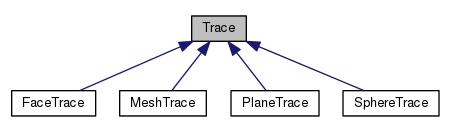
\includegraphics[width=\textwidth]{res/trace_inherit.png}
      \end{minipage}
    \end{figure}

    上图是\verb|Renderable|与\verb|Trace|的继承图,其中\verb|Trace|仅有三个子类是由于\verb|Mesh|返回\verb|FaceTrace|对象指针,
    \verb|KDTree|返回它所管理物体对应的\verb|Trace|对象指针.
    \verb|Renderable|类只有获取物体表面纹理及获取包围盒两种方法,
    \verb|Trace|类包括了判断相交、求交点、求交点法向、交点表面属性、交点前方介质密度等方法.

    这样做的好处是,由\verb|Trace|对象自己管理求交过程的中间结果,保留有用的结果以备其他方法使用.
    如判断是否相交时一些中间结果可能在计算交点距离时使用,交点法向方向有可能被计算纹理映射坐标时使用,
    这些中间结果是每一对$ (物体,光线)$特有的,又不该对外界暴露,因而用\verb|Trace|类将其封装.
    同时,这种设计使得同样的\verb|KDTree|类可以即在网格中又在整个空间中使用,并实现\verb|KDTree|的嵌套.

\end{enumerate}

kdtree

mainwindow

renderable

meshsimplifier

\subsection{视图导航}

\subsection{图形界面}
